\documentclass[12pt, letterpaper, preprint]{aastex63}
%%% This file is generated by the Makefile.
\newcommand{\giturl}{\url{https://github.com/changhoonhahn/eMaNu}}
\newcommand{\githash}{f673b16}\newcommand{\gitdate}{2019-07-23}\newcommand{\gitauthor}{changhoonhahn}

%\usepackage[breaklinks,colorlinks, urlcolor=blue,citecolor=blue,linkcolor=blue]{hyperref}
\usepackage{color}
\usepackage{amsmath}
\usepackage{natbib}
\usepackage{ctable}
\usepackage{bm}
\usepackage[normalem]{ulem} % Added by MS for \sout -> not required for final version
\usepackage{xspace}
\usepackage{csvsimple} 

\usepackage{graphicx}
\usepackage{pgfkeys, pgfsys, pgfcalendar}

% typesetting shih
\linespread{1.08} % close to 10/13 spacing
\setlength{\parindent}{1.08\baselineskip} % Bringhurst
\setlength{\parskip}{0ex}
\let\oldbibliography\thebibliography % killin' me.
\renewcommand{\thebibliography}[1]{%
  \oldbibliography{#1}%
  \setlength{\itemsep}{0pt}%
  \setlength{\parsep}{0pt}%
  \setlength{\parskip}{0pt}%
  \setlength{\bibsep}{0ex}
  \raggedright
}
\setlength{\footnotesep}{0ex} % seriously?

% math shih
\newcommand{\setof}[1]{\left\{{#1}\right\}}
\newcommand{\given}{\,|\,}
\newcommand{\lss}{{\small{LSS}}\xspace}

\newcommand{\lcdm}{$\Lambda$CDM} 
\newcommand{\Om}{\Omega_{\rm m}} 
\newcommand{\Ob}{\Omega_{\rm b}} 
\newcommand{\OL}{\Omega_\Lambda}
\newcommand{\smnu}{M_\nu}
\newcommand{\sig}{\sigma_8} 
\newcommand{\mmin}{M_{\rm min}}
\newcommand{\BOk}{\widehat{B}_0} 
\newcommand{\hmpc}{\,h/\mathrm{Mpc}}
\newcommand{\bfi}[1]{\textbf{\textit{#1}}}
\newcommand{\parti}[1]{\frac{\partial #1}{\partial \theta_i}}
\newcommand{\partj}[1]{\frac{\partial #1}{\partial \theta_j}}
\newcommand{\mpc}{h/{\rm Mpc}}

% specific to this project
\newcommand{\quij}{{\sc Quijote}}
\newcommand{\molino}{{\sc Molino}}
\newcommand{\planck}{{\em Planck}}
\newcommand{\kmax}{k_{\rm max}}
\newcommand{\Pg}{P^g} 
%\newcommand{\Pgl}{P^g_{\ell}} 
\newcommand{\Pgl}{P^g_0{+}P^g_2} 
\newcommand{\Bg}{B^g_0} 
\newcommand{\Phl}{P^h_{\ell}} 
\newcommand{\Bh}{B^h_0} 

\newcommand{\specialcell}[2][c]{%
  \begin{tabular}[#1]{@{}c@{}}#2\end{tabular}}
% text shih
\newcommand{\foreign}[1]{\textsl{#1}}
\newcommand{\etal}{\foreign{et~al.}}
\newcommand{\opcit}{\foreign{Op.~cit.}}
\newcommand{\documentname}{\textsl{Article}}
\newcommand{\equationname}{equation}
\newcommand{\bitem}{\begin{itemize}}
\newcommand{\eitem}{\end{itemize}}
\newcommand{\beq}{\begin{equation}}
\newcommand{\eeq}{\end{equation}}
\newcommand{\eg}{\emph{e.g.}}
\newcommand{\ie}{\emph{i.e.}}

%% collaborating
\newcommand{\todo}[1]{\marginpar{\color{red}TODO}{\color{red}#1}}
\definecolor{orange}{rgb}{1,0.5,0}
\newcommand{\ch}[1]{{\color{orange}{\bf CH:} #1}}

\begin{document}   %\sloppy\sloppypar\frenchspacing 

\title{Constraining $\smnu$ with the Bispectrum II: the Total Information Content of the Galaxy Bispectrum} 
%\date{\texttt{DRAFT~---~\githash~---~\gitdate~---~NOT READY FOR DISTRIBUTION}}

\newcounter{affilcounter}
\author{ChangHoon Hahn}
\altaffiliation{hahn.changhoon@gmail.com}
%\affil{Lawrence Berkeley National Laboratory, 1 Cyclotron Rd, Berkeley CA 94720, USA}
%\affil{Berkeley Center for Cosmological Physics, University of California, Berkeley, CA 94720, USA}
\affil{Department of Astrophysical Sciences, Princeton University, Peyton Hall, Princeton NJ 08544, USA} 

\author{Francisco Villaescusa-Navarro} 
\affil{Department of Astrophysical Sciences, Princeton University, Peyton Hall, Princeton NJ 08544, USA} 
\affil{Center for Computational Astrophysics, Flatiron Institute, 162 5th Avenue, New York, NY 10010, USA} 

%\author{...}

\begin{abstract}
    Massive neutrinos suppress the growth of structure on small scales %below their free-streaming scale 
    and leave an imprint on large-scale structure that can be measured to
    constrain their total mass, $\smnu$. With standard analyses of two-point
    clustering statistics, $\smnu$ constraints are severely limited by parameter
    degeneracies. \cite{hahn2020} demonstrated that the bispectrum, the
    next higher-order statistic, can break these degeneracies and dramatically
    improve constraints on $\smnu$ and other cosmological parameters. In this
    paper, we present the constraining power of the {\em redshift-space galaxy 
    bispectrum}, $\Bg$. We construct the
    \molino~suite of $75,000$ mock galaxy catalogs from the \quij~$N$-body simulations using the halo occupation distribution (HOD) model,
    which provides a galaxy bias framework well-suited for simulation-based
    approaches. Using these mocks, we present Fisher matrix forecasts for 
    $\{\Om$, $\Ob$, $h$, $n_s$, $\sig$, $\smnu\}$ and
    quantify, for the first time, the total information content of the $\Bg$
    down to nonlinear scales. For $\kmax{=}0.5\hmpc$, $\Bg$ improves constraints 
    on $\Om$, $\Ob$, $h$, $n_s$, $\sig$, and $\smnu$ by 2.8, 3.1, 3.8, 4.2,
    4.2, 4.7, and $5.6{\times}$ over the power spectrum, after marginalizing
    over HOD parameters. Even with priors from \planck, $\Bg$ improves all of 
    the cosmological constraints by $\gtrsim 2\times$. In fact, for $\Pgl$ and
    $\Bg$ out to $\kmax{=}0.5\hmpc$ with \planck~priors, we achieve a 
    $1\sigma$ $\smnu$ constraint of 0.048 eV, which is tighter than the current best 
    cosmological constraint. While effects such as survey geometry and assembly 
    bias will have an impact, these 
    %  the constraining power for galaxy surveys
    constraints are derived for $(1~h^{-1}{\rm Gpc})^3$, a substantially
    smaller volume than upcoming surveys. Therefore, we conclude that
    the galaxy bispectrum will significantly improve cosmological constraints
    for upcoming galaxy surveys --- especially for $\smnu$.
\end{abstract}

\keywords{
cosmology: cosmological parameters 
--- 
cosmology: large-scale structure of Universe.
---
cosmology: theory
}
\NewPageAfterKeywords

% --- intro ---
\section{Introduction} \label{sec:intro}
More than two decades ago, neutrino oscillation experiments discovered the lower
bound on the sum of neutrino masses ($\smnu \gtrsim 0.06$ eV) and confirmed
physics beyond the Standard Model~\citep{fukuda1998, forero2014, gonzalez-garcia2016}. 
Since then, experiments have sought to more precisely measure $\smnu$ in order
to distinguish between the `normal' and `inverted' neutrino mass hierarchy
scenarios and further reveal the physics of neutrinos. Upcoming laboratory 
experiments (\eg~double beta decay and tritium beta decay), however, will not
be sufficient to distinguish between the mass hierarchies~\citep{bonn2011, drexlin2013}.
Fortunately, complementary and more precise constraints on $\smnu$ can be
placed by measuring the effect of neutrinos on the expansion history and growth
of cosmic structure. 

In the early Universe, neutrinos are relativistic and contribute to the 
energy density of radiation. Later, as they become non-relativistic, 
they contribute to the energy density of matter. This transition affects 
the expansion history of the Universe and leaves imprints on the cosmic
microwave background~\citep[CMB;][]{lesgourgues2012, lesgourgues2014}. 
Massive neutrinos also impact the growth of structure. 
While neutrino perturbations are indistinguishable from cold dark matter (CDM)
perturbations on large scales, below their free-streaming scale, neutrinos 
do not contribute to the clustering and reduce the 
amplitude of the total matter power spectrum. They also reduce the growth 
rate of CDM perturbations at late times. This combined suppression of 
the small-scale matter power spectrum leaves measurable imprints 
on the CMB as well as large-scale structure~\citep[for further details see][]{lesgourgues2012, lesgourgues2014, gerbino2018}. 

%\todo{transition to why LSS neutrino mass measurement is important} (condensed version of paper 1) 
The tightest cosmological constraints on $\smnu$ currently come from 
combining CMB temperature and large angle polarization data from the 
\planck satellite with Baryon Acoustic Oscillation and CMB lensing: 
$\smnu < 0.13$ eV~\citep{planckcollaboration2018}. Future improvements
will likely continue to come from combining CMB data on large scales 
with clustering/lensing data on small scales and low redshifts, where 
the suppression of power by neutrinos is strongest~\citep{brinckmann2019}. 
But they will heavily rely on a better determination of $\tau$, the optical
depth of reionization since CMB experiments measure the combined quantity $A_s
e^{-2\tau}$~\citep{allison2015, liu2016, archidiacono2017}.
Major upcoming CMB experiments, however, are ground-based (\eg~CMB-S4) and 
will not directly constrain $\tau$~\citep{abazajian2016}. Meanwhile, proposed
future space-based experiments such as
LiteBIRD\footnote{http://litebird.jp/eng/} and 
LiteCOrE\footnote{http://www.core-mission.org/}, which have the greatest 
potential to precisely measure $\tau$, have yet to be confirmed. 

Despite the $\tau$ bottleneck in the near future, measuring the $\smnu$ imprint 
on the 3D clustering of galaxies provides a promising avenue for improving $\smnu$ constraints. 
Upcoming galaxy surveys such as DESI\footnote{https://www.desi.lbl.gov/}, 
PFS\footnote{https://pfs.ipmu.jp/}, EUCLID\footnote{http://sci.esa.int/euclid/}, 
and the Roman Space Telescope\footnote{https://roman.gsfc.nasa.gov/}, 
with the unprecedented cosmic volumes they will probe, 
have the potential to tightly constrain 
$\smnu$~\citep{audren2013, font-ribera2014, petracca2016, sartoris2016, boyle2018}.
Constraining $\smnu$ from 3D galaxy clustering, however, faces two major 
challenges: (1) accurate theoretical modeling beyond linear scales, for bias
tracers in redshift-space and (2) parameter degeneracies that limit the
constraining power of standard two-point clustering analyses. 

For the former, simulations have made huge strides in accurately modeling 
nonlinear structure formation with massive neutrinos~\citep[\eg][]{brandbyge2008, 
villaescusa-navarro2013, castorina2015, adamek2017, emberson2017, banerjee2018, 
villaescusa-navarro2018, villaescusa-navarro2019}. Moreover, new simulation-based
approaches to modeling such as `emulation' enable us to tractably exploit the accuracy of 
$N$-body simulations and analyze galaxy clustering on nonlinear scales beyond
traditional perturbation theory methods. Recent works have applied
these simulation-based approaches to analyze small-scale galaxy clustering with
remarkable success~\citep[\eg][]{heitmann2009, kwan2015, euclidcollaboration2018, lange2019, zhai2019, wibking2019}. 
These developments present the opportunity to significantly improve $\smnu$
constraints by unlocking the information content in nonlinear clustering, where
the impact of massive neutrinos is strongest~\citep[\eg][]{brandbyge2008,
saito2008, wong2008, saito2009, viel2010, agarwal2011, marulli2011, bird2012,
castorina2015, banerjee2016, upadhye2016}.

For the latter, parameter degeneracies such as the $\smnu$--$\sig8$
degeneracy pose serious limitations on constraining 
%\cite{villaescusa-navarro2018} recently used more than 1000 $N$-body
%simulations from the {\sc Hades} suite to examine the redshift-space matter and
%halo power spectrum.  They found that the imprint of $\smnu$ and $\sig$ on the
%redshift-space halo power spectrum are degenerate and differ by $< 1\%$. This
%$\smnu$ -- $\sig$ degeneracy poses a serious limitation on constraining 
$\smnu$ with the power spectrum~\citep{villaescusa-navarro2018}. However, 
information in the nonlinear regime cascades
from the power spectrum to higher-order statistics such as the bispectrum 
and help break these degeneracies~\citep{hahn2020}. Previous studies have already demonstrated the
potential of the bispectrum for improving cosmological parameter
constraints~\citep{sefusatti2005, sefusatti2006, chan2017, yankelevich2019,
agarwal2020}.
\cite{chudaykin2019}, in particular, included $\smnu$ in their forecast and
found that the bispectrum significantly improves constraints on $\smnu$.
However, none of these perturbation theory based forecast include the
constraining power on nonlinear scales. 

In \cite{hahn2020}, the previous paper of this series, we used 22,000 $N$-body
simulations from the \quij suite to quantify the total information content and
constraining power of the redshift-space halo bispectrum down to nonlinear scales. 
For $k_{\rm max}{=}0.5~\mpc$, we found that the bispectrum achieves $\Om$,
$\Ob$, $h$, $n_s$, and $\sig$ constraints 1.9, 2.6, 3.1, 3.6, and 2.6 times
tighter than the power spectrum. For $\smnu$, the bispectrum improved 
constraints by 5 times over the power spectrum. In this forecast, we marginalized 
over linear bias, $b_1$, and halo mass limit, $M_{\rm lim}$, parameters. We also found that the
improvements from the bispectrum are not impacted when we include quadratic 
and nonlocal bias parameters in the forecast. Nevertheless, \cite{hahn2020}
focused on the halo bispectrum. Actual constraints on $\smnu$, however, will be 
derived from the distribution of galaxies and therefore require a more 
realistic and complete galaxy bias model, which we provide in this paper.

In this work, we present the total information content and constraining power
of the {\em redshift-space galaxy bispectrum} down to $k_{\rm max}= 0.5~\hmpc$. For our galaxy
bias model, we use the halo occupation distribution (HOD) framework, which provides a
statistical prescription for populating dark matter halos with central and satellite
galaxies. The HOD model has been successful in reproducing the observed galaxy
clustering~\citep[\emph{e.g.}][]{zheng2005, leauthaud2012, tinker2013, zentner2016, vakili2019}. 
It is also the primary framework used in simulation-based clustering
analyses~\citep[\eg][]{mcclintock2018, zhai2019, lange2019, wibking2019}. 
We first construct 195,000 galaxy mock catalogs from the \quij $N$-body
simulations then use them to calculate Fisher matrix forecasts. Afterwards, we
present the constraining power of the galaxy bispectrum on $\smnu$ and other 
cosmological parameters after marginalizing over the HOD parameters. This work
is the second paper in a series that aims to demonstrate the potential for
simulation-based galaxy bispectrum analyses in constraining $\smnu$. Later in
the series, we will also present methods to tackle challenges that come with
analyzing the full galaxy bispectrum, such as data compression to reduce its
dimensionality. The series will culminate in fully simulation-based $\Pgl$ and
$\Bg$ reanalysis of SDSS-III BOSS. 

In Sections~\ref{sec:sims} and~\ref{sec:hod}, we describe the \quij $N$-body simulation 
suites and the HOD framework we use to construct galaxy mock catalogs from them. We then 
describe in Section~\ref{sec:methods}, how we measure the bispectrum and
calculate the Fisher forecasts of the cosmological parameters from the galaxy
mocks. Finally, in Section~\ref{sec:results}, we present the full information
content of the galaxy bispectrum and demonstrate how it significantly improves
the constraints on the cosmological parameters: $\Om$, $\Ob$, $h$, $n_s$,
$\sig$, and {\em especially} $\smnu$. 


% --- quijote ---
\section{HADES and Quijote Simulation Suites} \label{sec:hades} 
The HADES\footnote{https://franciscovillaescusa.github.io/hades.html} and Quijote 
suites are sets of, 42000 total, $N$-body simulations run on multiple cosmologies,
including those with massive neutrinos ($\smnu > 0$ eV). In this work, 
we use a subset of the HADES and Quijote simulations. Below, we briefly describe these simulations; 
a summary of the simulations can be found in Table~\ref{tab:sims}. 
The HADES simulations start from Zel'dovich approximated initial conditions 
generated at $z=99$ using the~\cite{zennaro2017a} rescaling method and follow 
the gravitational evolution of $N_{\rm cdm}=512^3$ CDM, plus $N_{\nu}=512^3$ 
neutrino particles for $\smnu > 0$ eV cosmologies, to $z=0$. They are run using 
the {\sc GADGET-III} TreePM+SPH code~\citep{springel2005} in a periodic 
$(1~h^{-1}{\rm Gpc})^3$ box. All of the HADES simulations share the following 
cosmological parameter values, which are in good agreement with Planck 
constraints~\cite{ade2016a}: $\Om{=}0.3175, \Ob{=}0.049, \OL{=}0.6825, n_s{=}0.9624, h{=}0.6711$, 
and $k_{\rm pivot} = 0.05~h{\rm Mpc}^{-1}$. 

The HADES suite includes $N$-body simulations with degenerate massive neutrinos 
of $\smnu = $ 0.06, 0.10, and 0.15 eV. These simulations are run using the 
``particle method'', where neutrinos are described as a collisionless 
and pressureless fluid and therefore modeled as particles, same as 
CDM~\citep{brandbyge2008,viel2010}. HADES also includes simulations with massless 
neutrino and different values of $\sigma_8$ to examine the $\smnu-\sigma_8$ 
degeneracy. The $\sigma_8$ values were chosen to match either $\sigma_8^m$ or 
$\sigma_8^{c}$ --- $\sigma_8$ computed with respect to total matter 
(CDM + baryons + $\nu$) or CDM + baryons --- of the massive neutrino simulations: 
$\sigma_8 = 0.822, 0.818, 0.807$, and $0.798$. Each model has $100$ independent 
realizations and we focus on the snapshots saved at $z = 0$. Halos closely 
trace the CDM+baryon field rather than the total matter field and neutrinos 
have negligible contribution to halo masses~\citep[\emph{e.g.}][]{ichiki2012, castorina2014, loverde2014, villaescusa-navarro2014}.
Hence, dark matter halos are identified in each realization using the Friends-of-Friends 
algorithm~\cite[FoF;][]{davis1985} with linking length $b=0.2$ on the CDM + baryon
distribution. We limit the halo catalogs to halos with masses above 
$M_{\rm lim} = 3.2\times 10^{13} h^{-1}M_\odot$. We refer readers
to~\cite{villaescusa-navarro2018} for more details on the HADES simulations. 

In addition to HADES, we use simulations from the Quijote suite, a
set of 42,000 $N$-body simulations that in total contain more than 8 trillion 
($8\times10^{12}$) particles over a volume of $42000 (h^{-1}{\rm Gpc})^3$. 
These simulations were designed to quantify the information content of 
different cosmological observables using Fisher matrix forecasting 
technique~(Section~\ref{sec:forecasts}). They are therefore designed to accurately 
calculate the covariance matrices of observables and the derivatives of observables with 
respect to cosmological parameters: 
$\Om$, $\Ob$, $h$, $n_s$, $\sig$, and $\smnu$.

To calculate covariance matrices, Quijote includes $N_{\rm cov}{=}15,000$ $N$-body 
simulations at a fiducial cosmology ($\Om{=}0.3175$, $\Ob{=}0.049$, $h{=}0.6711$, 
$n_s{=}0.9624$, $\sig{=}0.834$, and $\smnu{=}0.0$ eV). It also includes sets 
of 500 $N$-body simulations run at different cosmologies where only one parameter 
is varied from the fiducial cosmology at a time for the derivatives. Along $\Om$, 
$\Ob$, $h$, $n_s$, and $\sig$, the fiducial cosmology is adjusted by either a 
small step above or below the fiducial value: 
$\{\Om^{+}, \Om^{-}, \Ob^{+}, \Ob^{-}, h^+, h^-, n_s^{+}, n_s^{-}, \sig^{+}, \sig^-\}$ . 
Along $\smnu$, because $\smnu \ge 0.0$ eV and the derivative of certain observable 
with respect to $\smnu$ is noisy, Quijote includes sets of 500 simulations for 
$\smnu = 0.1$, 0.2, and 0.4 eV. Table~\ref{tab:sims} lists the cosmologies included 
in the Quijote suite. 

The intial conditions for all Quijote simulations were generated at $z=127$ using 
2LPT for simulations with massless neutrinos and the Zel’dovich approximation for 
massive neutrinos. Like HADES, the initial conditions of simulations with massive
neutrinos take their scale-dependent growth factors/rates into account using the
\cite{zennaro2017a} method. From the initial conditions, all of the simulations 
follow the gravitational evolution of $512^3$ dark matter particles, and $512^3$ 
neutrino particles for massive neutrino models, to $z=0$ using {\sc Gadget-III}
TreePM+SPH code (same as HADES). 
\ch{Halos are then identified using the same FoF scheme and mass limit as HADES. 
For the fiducial cosmology, the halo catalogs have ${\sim}156,000$ halos 
($\bar{n} \sim 1.56 \times 10^{-4}~h^3{\rm Gpc}^{-3}$) with $\bar{n} P_0(k=0.1)\sim 3.23$.}
% The simulations run at the fiducial cosmology for covariance matrix estimation are standard $N$-body simulations. However, the rest are paired fixed simulations, which greatly reduce cosmic variance without introducing bias for a large set of statistics~\citep{angulo2016,pontzen2016,villaescusa-navarro2018}.  We confirm that the paired fixed simulations do not introduce any bias for the redshift-space halo bispectrum (the observable we consider in this paper). 
We refer readers to Villaescusa-Navarro et al. (in preparation) for further details 
on the Quijote simulations.

\begin{figure}
\begin{center}
\includegraphics[width=0.9\textwidth]{figs/haloPlk_rsd_ratio.pdf}
    \caption{Impact of $\smnu$ and $\sig$ on the redshift-space halo power 
    spectrum monopole, $P_0$, and quadrupole, $P_2$, of the HADES simulation 
    suite. The $P_\ell$ measurements at each cosmology is
    averaged over 100 $N$-body realizations. $\smnu$ and $\sig$ produce 
    almost identical effects on halo clustering on small scales 
    ($k > 0.1\hmpc$). This degeneracy can be partially broken through 
    the quadrupole; however, {\em $\smnu$ and $\sig$ produce almost 
    the same effect on two-point clustering --- within a few percent}.
    }
\label{fig:plk}
\end{center}
\end{figure}


%%%%%%%%%%%%%%%%%%%%%%%%%%%%%%%%%%%%%%%%%%
% simulation table
%%%%%%%%%%%%%%%%%%%%%%%%%%%%%%%%%%%%%%%%%%
\begin{table}
\caption{Specifications of the HADES and Quijote simulation suites.} 
\begin{center}
\begin{tabular}{ccccccccc} \toprule
    Name  &$\smnu$ & $\Omega_m$ & $\Omega_b$ & $h$ & $n_s$ & $\sigma^m_8$ & $\sigma^c_8$ & realizations \\
      &({\footnotesize eV}) & & & & & ({\footnotesize $10^{10}h^{-1}M_\odot$}) & ({\footnotesize $10^{10}h^{-1}M_\odot$}) & \\[3pt] \hline\hline
    \multicolumn{9}{c}{HADES suite} \\ \hline
    Fiducial    & 0.0   & 0.3175 & 0.049 & 0.6711 & 0.9624 & 0.833 & 0.833 & 100 \\ 
                & 0.06  & 0.3175 & 0.049 & 0.6711 & 0.9624 & 0.819 & 0.822 & 100 \\ 
                & 0.10  & 0.3175 & 0.049 & 0.6711 & 0.9624 & 0.809 & 0.815 & 100 \\ 
                & 0.15  & 0.3175 & 0.049 & 0.6711 & 0.9624 & 0.798 & 0.806 & 100 \\ 
                & 0.0   & 0.3175 & 0.049 & 0.6711 & 0.9624 & 0.822 & 0.822 & 100 \\ 
                & 0.0   & 0.3175 & 0.049 & 0.6711 & 0.9624 & 0.818 & 0.818 & 100 \\ 
                & 0.0   & 0.3175 & 0.049 & 0.6711 & 0.9624 & 0.807 & 0.807 & 100 \\ 
                & 0.0   & 0.3175 & 0.049 & 0.6711 & 0.9624 & 0.798 & 0.798 & 100 \\[3pt]
    \hline \hline
    \multicolumn{9}{c}{Qujiote suite} \\ \hline
    Fiducial 	    & 0.0         & 0.3175 & 0.049 & 0.6711 & 0.9624 & 0.834 & 0.834 & 15,000 \\ 
    $\smnu^+$       & \underline{0.1}   & 0.3175 & 0.049 & 0.6711 & 0.9624 & 0.834 & 0.834 & 500 \\ 
    $\smnu^{++}$    & \underline{0.2}   & 0.3175 & 0.049 & 0.6711 & 0.9624 & 0.834 & 0.834 & 500 \\ 
    $\smnu^{+++}$   & \underline{0.4}   & 0.3175 & 0.049 & 0.6711 & 0.9624 & 0.834 & 0.834 & 500 \\ 
    $\Omega_m^+$    & 0.0   & \underline{ 0.3275} & 0.049 & 0.6711 & 0.9624 & 0.834 & 0.834 & 500 \\ 
    $\Omega_m^-$    & 0.0   & \underline{ 0.3075} & 0.049 & 0.6711 & 0.9624 & 0.834 & 0.834 & 500 \\ 
    $\Omega_b^+$    & 0.0   & 0.3175 & \underline{0.051} & 0.6711 & 0.9624 & 0.834 & 0.834 & 500 \\ 
    $\Omega_b^-$    & 0.0   & 0.3175 & \underline{0.047} & 0.6711 & 0.9624 & 0.834 & 0.834 & 500 \\ 
    $h^+$           & 0.0   & 0.3175 & 0.049 & \underline{0.6911} & 0.9624 & 0.834 & 0.834 & 500 \\ 
    $h^-$           & 0.0   & 0.3175 & 0.049 & \underline{0.6511} & 0.9624 & 0.834 & 0.834 & 500 \\ 
    $n_s^+$         & 0.0   & 0.3175 & 0.049 & 0.6711 & \underline{0.9824} & 0.834 & 0.834 & 500 \\ 
    $n_s^-$         & 0.0   & 0.3175 & 0.049 & 0.6711 & \underline{0.9424} & 0.834 & 0.834 & 500 \\ 
    $\sigma_8^+$    & 0.0   & 0.3175 & 0.049 & 0.6711 & 0.9624 & \underline{0.849} & \underline{0.849} & 500 \\ 
    $\sigma_8^-$    & 0.0   & 0.3175 & 0.049 & 0.6711 & 0.9624 & \underline{0.819} & \underline{0.819} & 500 \\[3pt]
    \hline
\end{tabular} \label{tab:sims}
\end{center}
    {\bf \em Top}: The HADES suite includes sets of 100 $N$-body simulations with degenerate massive neutrinos 
    of $\smnu = $ 0.06, 0.10, and 0.15 eV as well as sets of simulations with $\smnu = 0.0$ eV and 
    $\sigma_8 = $ 0.822, 0.818, 0.807, and 0.798 to examine the $\smnu-\sigma_8$ degeneracy. 
    {\bf \em Bottom}: The Quijote suite includes 15,000 $N$-body simulations at the fiducial 
    cosmology to accurately estimate the covariance matrices. It also includes sets of 500 
    simulations at different cosmologies, where only one parameter is varied from the fiducial 
    value (underlined), to estimate derivatives of observables along the cosmological parameters.
\end{table}
%%%%%%%%%%%%%%%%%%%%%%%%%%%%%%%%%%%%%%%%%%


% --- hod ---
\begin{figure}
\begin{center}
    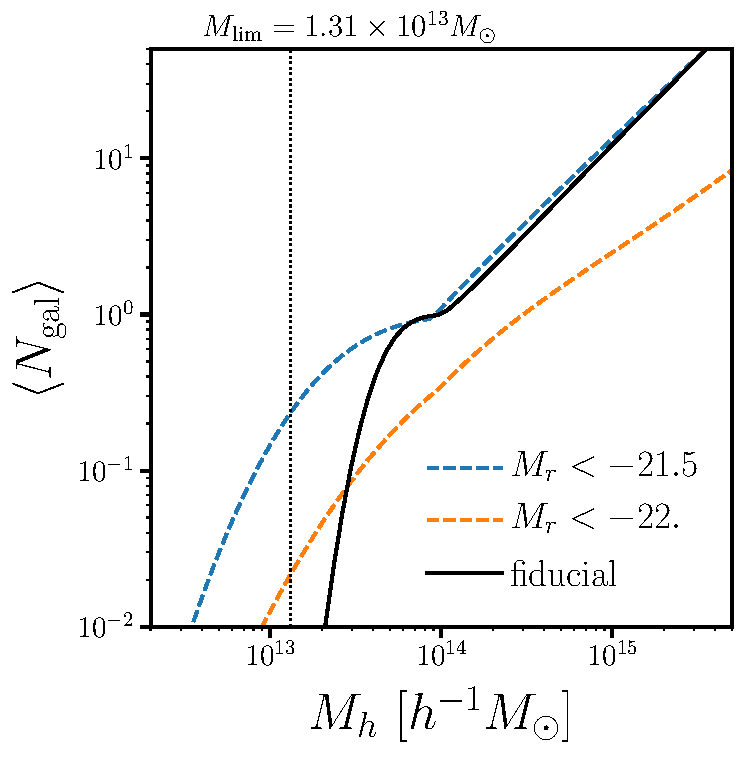
\includegraphics[width=0.75\textwidth]{figs/hod_fid.pdf} 
    \caption{

    }\label{fig:hod}
\end{center}
\end{figure}

\section{Halo Occupation Distribution} \label{sec:hod}  
We're interested in quantifying the information content of the galaxy 
bispectrum. With a perturbation theory approach, this would involve 
incorporating a bias model for galaxies~\citep[\emph{e.g.}][]{sefusatti2006, yankelevich2019, chudaykin2019}. 
Instead, for our simulation driven approach, we use the halo occupation 
distribution (HOD) framework~\citep[\emph{e.g.}][]{zheng2005,leauthaud2012,tinker2013,zentner2016,vakili2019}. 
The HOD model specifies how 

\bitem
\item description of HODs in general and how we're going to use them our bias model. 
    This is the framework used to construct simulated mock catalogs and used 
    ubiquitously in galaxy clustering analyses. Moreover, it's used for emulator 
    set ups (Aemulus), which as we mention earlier is the only hopes for accurately 
    modeling the high k.
\item We use the standard \cite{zheng2007} model, which has been used extensively. 
    Discuss the obvious shortcomings of the model. However, \cite{vakili2019} did not 
    find strong evidence for assembly bias and we're going for simplicity here. 
\item description of the halo mass constraints we're dealing with and how this prevents 
    us from directly using best-fit HOD parameters from the literature. In fact, due
    to this constraint we modify the HOD parameters.
\item plots showing how our HOD choice compares to HODs of the SDSS samples. Some handwavy
    arguments about how it shouldn't matter too much. 
\eitem

% --- excerpt from Hahn et al. (2017) --- 
%The foundation of HOD predictions is the halo model of LSS, that is, collapsed dark matter halos are biased tracers of the underlying cos- mic density field (Press & Schechter 1974; Bond et al. 1991; Cooray & Sheth 2002). The HOD specifies how the dark matter halos are populated with galaxies by modeling the probability that a given halo hosts N galaxies subject to some observational selection criteria (Lemson & Kauffmann 1999; Seljak 2000; Scoccimarro et al. 2001; Berlind & Wein- berg 2002; Zheng et al. 2005). This statistical prescription for connecting galaxies to halos has been remarkably successful in reproducing the galaxy clustering, galaxy–galaxy lensing, and other observational statistics (Rodr ́ıguez-Torres et al. 2015; Miyatake et al. 2015), and is a useful framework for constraining cosmological parameters (van den Bosch et al. 2003; Tinker et al. 2005; Cacciato et al. 2013; More et al. 2013) as well as galaxy evolution models (Conroy & Wech- sler 2009; Tinker et al. 2011; Leauthaud et al. 2012; Behroozi et al. 2013b; Tinker et al. 2013, Walsh et al. in preparation).

% --- excerpt from Zhai et al. (2018) --- 
%Retrieving information from these scales has been a goal of modern cosmology, but it has also been a challenge. Non- linear dynamics of dark matter are captured with excellent precision in modern cosmological N-body simulations (see, e.g., Klypin et al. 2011, 2016). The challenge of constraining cosmology with such simulations is two-fold: (1) an accu- rate and flexible model of the galaxy bias is required, and (2) one needs to be able to properly sample cosmological pa- rameter space, which becomes computationally intractable for a standard Monte Carlo Markov Chain analysis. Be- cause of these limitations, the amount of information that is extractable from small-scale galaxy clustering is simply unknown. The measurement precision of the data is orders of magnitude higher than at large scales, but the theoretical complexity increases significantly. How much information is recoverable after accounting for all possibilities in galaxy bias? In this paper, for the case of RSD, we will show that af- ter marginalizing over numerous galaxy bias parameters and incorporating the theoretical uncertainty in the galaxy clus- tering model, it is still possible to extract more constraining power from growth of structure measurements than what is achievable using perturbation theory on large scales.
%To solve problem (1), we use the halo occupation distri- bution (HOD; Berlind & Weinberg 2002; Peacock & Smith 2000; Seljak 2000; Benson et al. 2000; White et al. 2001; Cooray & Sheth 2002). The HOD approaches galaxy bias by quantifying the statistical relationship between galaxies and dark matter halos. In its most basic form, the HOD is mostly determined by the probability distribution P(N|M), the prob- ability that a halo of mass M contains N galaxies of a given class. Once P(N|M) is combined with prescriptions for spa- tial and velocity bias of galaxies within halos, this model of- fers nearly a complete description of the spatial distribution of galaxies for a given halo population. This simple approach of P(N|M), however, ignores the possibility that N may de- pend on some secondary halo property. If this halo property is correlated with the spatial distribution of halos, this could create a ‘galaxy secondary bias’ (also known as galaxy as- sembly bias) that would have to be incorporated in the prob- ability distribution in order to create a fully descriptive HOD (Sheth & Tormen 2004; Gao et al. 2005; Harker et al. 2006; Wechsler et al. 2006). The optimal method for incorporating galaxy assembly bias into the HOD, and tests against models that contain these effects, is left to another paper (McLaugh- lin et al. 2018). Our emphasis here is on determining the to- tal constraining power and the scales from which these con- straints come, under the assumption that the assumed HOD approach is sufficient for modeling galaxy bias.
 

% --- methods ---
\section{Bispectrum and Cosmological Parameter Forecasts} \label{sec:methods}
We measure the bispectrum and calculate the parameter constraints using the same methods as
\cite{hahn2020}. For further details, we therefore refer readers to \cite{hahn2020}. 

To measure $\Bg$, we use a Fast Fourier Transform (FFT) based estimator similar to
the ones described in \cite{sefusatti2005}, \cite{scoccimarro2015}, and
\cite{sefusatti2016}. Galaxy positions are first interpolated onto a grid,
$\delta(\bfi{x})$, using a fourth-order interpolation scheme, which has advantageous
anti-aliasing properties that allow unbiased measurements up to the Nyquist
frequency~\citep{hockney1981, sefusatti2016}. After Fourier transforming 
$\delta(\bfi{x})$ to get $\delta(\bfi{k})$, we measure the bispectrum monopole:  
\beq \label{eq:bk} 
\Bg(k_1, k_2, k_3) = \frac{1}{V_B} \int\limits_{k_1}{\rm d}^3q_1
\int\limits_{k_2}{\rm d}^3q_2 \int\limits_{k_3}{\rm d}^3q_3~\delta_{\rm
D}({\bfi q_{123}})~\delta({\bfi q_1})~\delta({\bfi q_2})~\delta({\bfi q_3}) -
B^{\rm SN}_0.
\eeq
$\delta_D$ is the Dirac delta function, $V_B$ is the normalization factor
proportional to the number of triplets that can be found in the $k_1, k_2, k_3$
triangle bin, and $B^{\rm SN}_0$ is the correction term for the Poisson shot
noise. Throughout the paper, we use $\delta(\bfi{x})$ grids with $N_{\rm grid}
= 360$ and triangle configurations defined by $k_1, k_2, k_3$ bins of width
$\Delta k = 3 k_f = 0.01885\hmpc$, where $k_f = 2\pi/(1000~h^{-1}{\rm Mpc})$. 

In Figure~\ref{fig:bgh}, we present the redshift-space galaxy power spectrum multipoles 
($\Pgl$; left) and bispectrum ($\Bg$; right) of the fiducial HOD galaxy catalog (blue). The $\Pgl$ and 
$\Bg$ are averaged over one set of HOD realizations run on 15,000 $N$-body
\quij simulations at the fiducial cosmology. In the left panel, we
plot both the power spectrum monopole ($\ell = 0$; solid) and quadrupole 
($\ell = 2$; dashed). In the right panel, we plot $\Bg$ for all 1898 triangle
configurations with $k_1, k_2, k_3 \ge k_{\rm max} = 0.5\hmpc$. The configurations 
are ordered by looping through $k_3$ in the inner most loop and $k_1$ in the outer
most loop satisfying $k_1 \le k_2 \le k_3$. For comparison, we include the
redshift-space halo power spectrum and bispectrum at the fiducial cosmology 
from \cite{hahn2020} (black). 

\begin{figure}
\begin{center}
    \includegraphics[width=\textwidth]{figs/PBg_reg.pdf} 
    \caption{The redshift-space galaxy power spectrum multipoles ($\Pgl$; left)
    and bispectrum monopole ($\Bg$; right) of the fiducial HOD galaxy catalog (blue).
    The $\Pgl$ and $\Bg$ are averaged over one set of HOD realizations run on
    15,000 $N$-body \quij simulations measured using the same FFT-based estimator as \cite{hahn2020}. In the 
    left panel, we plot both the power spectrum monopole ($\ell = 0$; solid) and quadrupole 
    ($\ell = 2$; dashed). In the right panel, we plot $\Bg$ for all 1898 triangle
    configurations with $k_1, k_2, k_3 \ge k_{\rm max} = 0.5\hmpc$. The
    configurations are ordered by looping through $k_3$ in the inner most loop
    and $k_1$ in the outer most loop satisfying $k_1 \le k_2 \le k3$.
    We include for comparison the \cite{hahn2020} halo $\Phl$ and $\Bh$ at the 
    fiducial cosmology (black). %We note that the fiducial galaxy catalog has $\bar{n}_g \sim 1.63\times 10^{-4}~h^3{\rm Gpc}^{-3}$ and linear bias of $b_g \sim 2.55$.
    }
\label{fig:bgh}
\end{center}
\end{figure}

To estimate the constraining power of $\Pgl$ and $\Bg$, we use Fisher information
matrices, which have been ubiquitously used in
cosmology~\citep[\emph{e.g.}][]{jungman1996,tegmark1997,dodelson2003,heavens2009,verde2010}: 
\beq 
F_{ij} = - \bigg \langle \frac{\partial^2 \mathrm{ln} \mathcal{L}}{\partial \theta_i \partial \theta_j} \bigg \rangle,
\eeq
As in \cite{hahn2020}, we assume that the $\Bg$ lieklihood is Gaussian and
neglect the covariance derivative term~\citep{carron2013} and estimate the
Fisher matrix as 
\beq \label{eq:fisher}
F_{ij} = \frac{1}{2}~\mathrm{Tr} \Bigg[\bfi{C}^{-1}
\left(\parti{\Bg}\partj{\Bg}^T + \parti{\Bg}^T \partj{\Bg} \right)\Bigg].
\eeq
We derive the covariance matrix, $\bfi{C}$, using the $15,000$ galaxy catalogs
at the fiducial cosmology. The derivatives along the cosmological and HOD
parameters, $\partial \Bg/\partial \theta_i$, are estimated using finite
difference. For all parameters besides $\smnu$, we estimate 
\beq 
\frac{\partial \Bg}{\partial \theta_i} \approx \frac{\Bg(\theta_i^{+})-\Bg(\theta_i^{-})}{\theta_i^+ - \theta_i^-}, 
\eeq
where $\Bg(\theta_i^{+})$ and $\Bg(\theta_i^{-})$ are the average bispectrum of the 
$7,500$ realizations at $\theta_i^{+}$ and $\theta_i^{-}$, the HOD and  
cosmological parameter values above and below the fiducial parameters.  
For $\smnu$, where the fiducial value is 0.0 eV, we use the galaxy catalogs 
at $\smnu^+$, $\smnu^{++}$, $\smnu^{+++}=0.1, 0.2, 0.4$ eV (Table~\ref{tab:sims}) 
to estimate 
\beq \label{eq:dbkdmnu} 
\frac{\partial \Bg}{\partial \smnu} \approx \frac{-21 \Bg(\theta_{\rm fid}^{\rm ZA}) + 
32 \Bg(\smnu^{+}) - 12 \Bg(\smnu^{++}) + \Bg(\smnu^{+++})}{1.2}, 
\eeq
which provides a $\mathcal{O}(\delta \smnu^2)$ order approximation. 
Since the simulations at $\smnu^+$, $\smnu^{++}$, and $\smnu^{+++}$ are generated 
from Zel'dovich initial conditions, we use simulations at the fiducial cosmology 
also generated from Zel'dovich initial conditions ($\theta_{\rm fid}^{\rm ZA}$). 
We emphasize that our simulation-based approach with galaxy catalogs constructed from
$N$-body simulations is essential for accurately quantifying the constraining power
of our observables beyond the limitations of analytic methods down to the nonlinear regime.


% --- results ---
%%%%%%%%%%%%%%%%%%%%%%%%%%%%%%%%%%%%%%%%%%
% forecast table
%%%%%%%%%%%%%%%%%%%%%%%%%%%%%%%%%%%%%%%%%%
\begin{table}
    \caption{Marginalized Fisher parameter constraints from the redshift-space 
    $P_\ell$, $B_0$, and $P_\ell$ + $B_0$. We list constraints for cosmological 
    parameters $\smnu$, $\Omega_m$, $\Omega_b$, $h$, $n_s$, and $\sig$ as well 
    as HOD and nuisance parameters.} 
\begin{center} 
    \begin{tabular}{c|ccc|ccc} \hline
        & \multicolumn{3}{c}{$\kmax=0.2~\hmpc$} & \multicolumn{3}{c}{$\kmax=0.5~\hmpc$} \\ %& & $\kmax=0.2$ & & & $\kmax=0.5$ & \\
        & $P_\ell$ & $B_0$ & $P_\ell + B_0$ & $P_\ell$ & $B_0$ & $P_\ell + B_0$ \\[3pt] \hline 
$M_\nu$     &  0.795 (0.132) & 0.313 (0.123) & 0.282 (0.098) & 0.334 (0.112) & 0.073 (0.055) & 0.071 (0.048)  \\
$\Omega_m$  &  0.061 (0.021) & 0.047 (0.021) & 0.030 (0.014) & 0.037 (0.017) & 0.018 (0.012) & 0.013 (0.008)  \\
$\Omega_b$  &  0.027 (0.002) & 0.017 (0.002) & 0.013 (0.001) & 0.015 (0.002) & 0.006 (0.001) & 0.005 (0.001)  \\
$h$         &  0.351 (0.014) & 0.204 (0.014) & 0.157 (0.010) & 0.178 (0.011) & 0.052 (0.008) & 0.047 (0.006)  \\
$n_s$       &  0.427 (0.005) & 0.230 (0.005) & 0.165 (0.005) & 0.206 (0.005) & 0.053 (0.005) & 0.049 (0.004)  \\
$\sigma_8$  &  0.209 (0.029) & 0.116 (0.027) & 0.053 (0.023) & 0.089 (0.025) & 0.034 (0.014) & 0.021 (0.012)  \\ [3pt] \hline
$\log M_{\rm min}$ &  1.435 (1.061) & 0.499 (0.442) & 0.335 (0.210) & 0.457 (0.258) & 0.114 (0.100) & 0.089 (0.070)  \\
$\sigma_{\log M}$ &  3.072 (2.390) & 1.090 (0.926) & 0.712 (0.506) & 0.963 (0.655) & 0.215 (0.204) & 0.174 (0.140)  \\
$\log M_0$ &  2.257 (1.845) & 1.387 (1.341) & 0.431 (0.386) & 0.547 (0.361) & 0.261 (0.232) & 0.088 (0.079)  \\
$\alpha$ &  0.749 (0.592) & 0.309 (0.294) & 0.170 (0.167) & 0.257 (0.180) & 0.082 (0.073) & 0.034 (0.033)  \\
$\log M_1$ &  0.819 (0.691) & 0.434 (0.408) & 0.244 (0.149) & 0.193 (0.119) & 0.115 (0.113) & 0.071 (0.056)  \\
        [3pt]
\hline                                 
\end{tabular} \label{tab:forecast}
\end{center}
{$^*$ constraints with \planck priors in parentheses}
\end{table}

%%%%%%%%%%%%%%%%%%%%%%%%%%%%%%%%%%%%%%%%%%
% kmax = 0.2 
% P sigmas 0.06094, 0.02654, 0.35148, 0.42714, 0.20940, 0.79540, 1.43526, 3.07160, 2.25686, 0.74927, 0.81883
% B sigmas 0.04670, 0.01718, 0.20409, 0.23048, 0.11592, 0.31323, 0.49926, 1.09044, 1.38728, 0.30865, 0.43437
% P+B sigmas 0.03005, 0.01329, 0.15669, 0.16504, 0.05316, 0.28209, 0.33499, 0.71162, 0.43062, 0.16962, 0.24399
% kmax = 0.5
% P sigmas 0.03657, 0.01520, 0.17803, 0.20553, 0.08940, 0.33439, 0.45684, 0.96282, 0.54733, 0.25698, 0.19286
% B sigmas 0.01837, 0.00552, 0.05250, 0.05292, 0.03419, 0.07251, 0.11429, 0.21538, 0.26110, 0.08198, 0.11527
% P+B sigmas 0.01316, 0.00489, 0.04690, 0.04942, 0.02118, 0.07055, 0.08901, 0.17434, 0.08820, 0.03411, 0.07144
%%%%%%%%%%%%%%%%%%%%%%%%%%%%%%%%%%%%%%%%%%
% kmax = 0.2 with planck 
% P sigmas 0.02064, 0.00210, 0.01398, 0.00524, 0.02926, 0.13204, 1.06089, 2.38989, 1.84519, 0.59186, 0.69080
% B sigmas 0.02064, 0.00207, 0.01392, 0.00534, 0.02697, 0.12295, 0.44195, 0.92590, 1.34132, 0.29397, 0.40759
% P+B sigmas 0.01439, 0.00147, 0.00987, 0.00478, 0.02269, 0.09754, 0.21031, 0.50593, 0.38573, 0.16727, 0.14908
%%%%%%%%%%%%%%%%%%%%%%%%%%%%%%%%%%%%%%%%%%
\begin{figure}
    \begin{center}
        \includegraphics[width=\textwidth]{figs/Fisher_p02bk_dmnu_fin_kmax0_50_seed0to4.pdf}
        \caption{Fisher matrix constraints for $\smnu$ and other cosmological
        parameters for the redshift-space galaxy $\Pgl$ (blue), $\Bg$
        (green), and combined $\Pgl$ and $\Bg$ (orange) for $k_{\rm max} =
        0.5\hmpc$. Our forecasts marginalizes over the \cite{zheng2007}
        HOD parameters: $M_{\rm min}, \sigma_{\log M}, \log M_0, \alpha \log
        M_1$ (bottom panels). The contours mark the $68\%$ and $95\%$
        confidence intervals. The bispectrum substantially improves
        constraints on all of the cosmological parameters over the power
        spectrum. $\Om$, $\Ob$, $h$, $n_s$, and $\sig$ constraints improve by factors
        of 2.8, 3.1, 3.8, 4.2, and 4.2, respectively. For $\smnu$, the
        bispectrum improves $\sigma_{\smnu}$ from 0.3344 to 0.0706 eV --- over
        a factor of $\sim5$ improvement over the power spectrum.
        }
        \label{fig:forecast}
    \end{center}
\end{figure}

\begin{figure}
    \begin{center}
        \includegraphics[width=\textwidth]{figs/Fisher_kmax_p02bk_dmnu_fin_seed0to4.pdf}
        \caption{Marginalized $1\sigma$ constraints, $\sigma_\theta$, of the
        cosmological parameters $\Om$, $\Ob$, $h$, $n_s$, $\sig$, and $\smnu$
        as a function of $k_{\rm max}$ for the redshift-space $\Pgl$ (blue)
        and combined $\Pgl + \Bg$ (orange). Even after marginalizing over
        HOD parameters (Eq.~\ref{eq:hod_fid}), the galaxy bispectrum {\em
        significantly} improves cosmological parameter constraints above
        $k_{\rm max} > 0.1\hmpc$. Constraints from $\Pgl$ and
        $\Pgl + \Bg$ improve with higher $k_{\rm max}$. {\em Throughout 
        $0.2 < k_{\rm max} < 0.5$, including the bispectrum improves 
        $\{\Om, \Ob, h, n_s, \sig, \smnu\}$ constraints by factors of ${>}2$.} When we include 
        \planck priors (dotted), the improvement from $\Bg$ is even more
        evident. The constraining power of $\Pgl$ complete
        saturates for $\kmax \gtrsim 0.12\hmpc$. Adding $\Bg$ not only 
        improves constraints, but the constraints continue to improve for
        higher $k_{\rm max}$. At $k_{\rm max} = 0.2$ and $0.5\hmpc$, the $\Pgl
        + \Bg$ improves the $\smnu$ constraint by 1.4 and $2.3\times$ over $\Pgl$. 
        We emphasize that the constraints above are for $1~({\rm Gpc}/h)^3$ box
        and thus underestimate the constraining power of upcoming galaxy
        clustering surveys.
        }
        \label{fig:kmax_forecast}
    \end{center}
\end{figure}

\section{Results} \label{sec:results} 
We present the Fisher matrix constraints for $\smnu$ and other cosmological
parameters from the redshift-space galaxy $\Pgl$ (blue), $\Bg$ (green), and 
combined $\Pgl + \Bg$ (orange) in Figure~\ref{fig:forecast}. These
constraints marginalize over the \cite{zheng2007} HOD parameters %$\{M_{\rm min}, \sigma_{\log M}, \log M_0, \alpha \log M_1 \}$ 
(bottom panels) and extends to $k_{\rm max} = 0.5\hmpc$. The contours mark the $68\%$ and
$95\%$ confidence intervals. With the redshift-space $\Pgl$
alone, we derive the following $1\sigma$ constraints for $\{\Om, \Ob, h, n_s,
\sig, \smnu\}$: 
0.037, 0.015, 0.178, 0.206, 0.089, and 0.334.
With the redshift-space $\Bg$ alone, we get: 
0.018, 0.006, 0.052, 0.053, 0.034, and 0.073.
{\em The galaxy bispectrum produces tighter constraints on all cosmological
parameters over the power spectrum}.

Furthermore, we find that by combining $\Pgl$ and $\Bg$, we derive even better
constraints by breaking a number of parameter degeneracies. Among the cosmological 
parameters, in addition to breaking the $\sig - \smnu$ degeneracy, which limits
power spectrum analyses, the $\Om-\sig$ degeneracy is also broken and leads to
significant improvements in both $\Om$ and 
$\sig$ constraints. Meanwhile, for the HOD parameters, degeneracies with 
$\log M_0$, $\alpha$, and $\log M_1$ are substantially reduced. 
Combining $\Pgl$ and $\Bg$, we get the following $1\sigma$ constraints for 
 $\Om$, $\Ob$, $h$, $n_s$, $\sig$, and $\smnu$: 
0.013, 0.005, 0.047, 0.049, 0.021, and 0.071.
{\em With $\Pgl$ and $\Bg$ combined, we improve $\Om$, $\Ob$, $h$,
$n_s$, and $\sig$ constraints by factors of 2.8, 3.1, 3.8, 4.2, and 4.2
and $\smnu$ constraint by a factor of 4.7 over the $\Pg$ constraints}

In Figure~\ref{fig:kmax_forecast}, we present the marginalized $1\sigma$
constraints, $\sigma_\theta(\kmax)$, of the cosmological parameters $\Om$,
$\Ob$, $h$, $n_s$, $\sig$, and $\smnu$ as a function of $\kmax$ for $\Pgl$
(blue) and the combined $\Pgl + \Bg$ (orange). Again, these constraints are
marginalized over the \cite{zheng2007} HOD parameters. For both $\Pgl$ and
$\Pgl + \Bg$, parameter constraints expectedly improve as
we include higher $\kmax$. More importantly, {\em the galaxy bispectrum significantly 
improves cosmological parameter constraints throughout $\kmax > 0.1\hmpc$
and not only at high $\kmax$}. Even for $\kmax\sim 0.2\hmpc$, including 
$\Bg$ improves $\Om$, $\Ob$, $h$, $n_s$, $\sig$ and $\smnu$ constraints by 
factors of 2.0, 2.0, 2.2, 2.6, 3.9, and 2.8.

In Figure~\ref{fig:kmax_forecast}, we also present $\sigma_\theta(\kmax)$ for
$\Pgl$ (blue dashed) and $\Pgl + \Bg$ 
(orange dashed) {\em with priors from Planck}. Once we include \planck priors,
$\Pgl$ constraints do not significantly improve for $\kmax \gtrsim 0.12\hmpc$.
On the other hand, the constraints from $\Pgl + \Bg$ continues to improve for $\kmax > 0.15\hmpc$. 
At $\kmax=0.2\hmpc$, $\Bg$ improves the $\Pgl$ + \planck priors constraints on  
$\Om$, $\Ob$, $h$, $n_s$, $\sig$ and $\smnu$ constraint by factors of
1.4, 1.4, 1.4, 1.1, 1.3, and $1.4\times$.
At $\kmax = 0.5\hmpc$, $\Bg$ improves the $\Pgl$ + \planck priors constraints on  
$\Om$, $\Ob$, $h$, $n_s$, $\sig$ and $\smnu$ constraint by factors of 
2.0, 2.1, 1.9, 1.2, 2.2, and $2.3\times$.
Therefore, even with \planck priors, the galaxy bispectrum significantly improves cosmological 
constraints. In fact, we emphasize that the constraints in Figure~\ref{fig:kmax_forecast} 
are for a $1~({\rm Gpc}/h)^3$ box, a much smaller cosmic volume than upcoming
galaxy redshift surveys (\eg~DESI, Euclid). Our forecasts with \planck priors
{\em underestimate} the constraining power contribution from galaxy clustering 
that we expect from upcoming surveys.  With more constraining power coming 
from galaxy clustering, improvements from including $\Bg$ to $\Pgl$ and \planck
will be larger.

%The improvements of $\Bg$ come from breaking parameter degeneracies. 
%Most noteably, $\Om$ and $\sig$ degeneracies are broken by
%$\Pgl + \Bg$, which improves $\Om - \sig$, $\Om - \smnu$, $\sig-\smnu$ that we care about. 

% comparison to literature 
% ------------------------
% comparison to halo forecast
% SN kmax=0.20: Pg:92.984343, Bg:24.182641, Ph:121.561879, Bh:34.068850
% SN kmax=0.51: Pg:140.263416, Bg:30.561088, Ph:143.901659, Bh:75.042306
In the previous paper of the series~\citep{hahn2020}, we presented the full
information content of the redshift-space halo bispectrum, $\Bh$. For $\Bh$ to
$\kmax=0.5\hmpc$, \cite{hahn2020} derived $1\sigma$ constraints of 
0.012, 0.004, 0.04, 0.036, 0.014, and 0.057 
for $\Om$, $\Ob$, $h$, $n_s$, $\sig$ and $\smnu$. In comparison, we find constraints of 
0.018, 0.006, 0.052, 0.053, 0.034, and 0.073 
for $\Bg$ to $\kmax=0.5\hmpc$ (Table~\ref{tab:forecast}). 
$\Bg$ produces overall broader constraints on the cosmolgoical parameters. This
is the same for $\kmax=0.2\hmpc$. A comparison of the signal-to-noise ratios
(SNR) of $\Bg$ and $\Bh$, estimated from the covariance
matrix~\citep[\eg][]{sefusatti2005,sefusatti2006,chan2017}, also confirm the lower
constraining power of $\Bg$. Furthermore, while both $\Bh$ and $\Bg$ SNRs increase 
at higher $\kmax$, however the increase is lower for $\Bg$ than $\Bh$.
Marginalizing over HOD parameters reduces some of the constraining power of 
the bispectrum. Fingers-of-god (FoG), the elongation of satellite galaxies
in redshift-space along the line-of-sight due to their virial velocities inside 
halos, also contributes to this reduction. 
Nevertheless, $\Bg$ significantly improves parameters constraints over $\Pgl$.
In fact, marginalizing over HOD parameters and FoG reduces the constraining
power of the power spectrum more than the bispectrum. Therefore, {\em we find 
larger improvements in the parameter constraints from $\Bg$ over $\Pgl$ than
from $\Bh$ over $\Phl$}.

%comparison to the literature.
Other previous works have also quantified the information content of the
bispectrum:~\citep[\eg][]{scoccimarro2004, sefusatti2006, sefusatti2007,
song2015, tellarini2016, yamauchi2017a, karagiannis2018, yankelevich2019,
chudaykin2019, coulton2019, reischke2019}. 
We focus our comparison to \cite{sefusatti2006}, \cite{yankelevich2019}, 
and \cite{chudaykin2019}, which provide bispectrum forecasts for full sets of
cosmological parameters.
\cite{sefusatti2006} present \lcdm~forecasts for a joint likelihood analysis of
$\Bg$ with $\Pg$ and WMAP. For $\kmax = 0.2\hmpc$, they find that including
$\Bg$ improves constraints on $\Om$, $\Ob$, $h$, $n_s$, and $\sig$ by 1.6, 1.2,
1.5, 1.4, and 1.5 times from the $\Pg$ and WMAP constraints. In comparison, for 
$\kmax = 0.2\hmpc$ and with \planck priors, we find $\Bg$ improves constraints
by  1.5, 1.4, 1.4, 1.1, and $1.3\times$, which is in good agreement. There are,
however, some significant differences between our analyses. First, \cite{sefusatti2006} 
uses the WMAP likelihood while we use priors from {\em Planck}. Furthermore, 
in our simulation-based approach, we marginalizes over the HOD parameters
whereas \cite{sefusatti2006} marginalize over the linear and quadratic bias
terms ($b_1, b_2$) in their perturbation theory approach. Nevertheless, our
results are consistent with the improvement \cite{sefusatti2006} find in
parameter constraints with $\Bg$. 

%comparison to the Yankelevic 
Next, \cite{yankelevich2019} present \lcdm, $w$CDM and $w_0w_a$CDM Fisher
forecasts for a Euclid-like survey\cite{laureijs2011} over $0.65 < z < 2.05$.
Focusing only on their \lcdm~forecasts, they find that for $\kmax = 0.15\hmpc$, 
$\Pg+\Bg$ produces constraints on $\Omega_{\rm cdm}$, $\Ob$, $A_s$, $h$, $n_s$ 
that are ${\sim}1.3\times$ tighter than $\Pg$ alone. In contrast, we find even
at $\kmax=0.15\hmpc$ significantly larger improvement in the parameter constraints 
from including $\Bg$. We note that \cite{yankelevich2019} present forecasts for
a significantly different galaxy sample. For instance, their $z = 0.7$ redshift
bin has $\bar{n}_g = 2.76 \times 10^{-3}~h^3{\rm Gpc}^{-3}$ and linear bias of
$b_g = 1.18$. Meanwhile our galaxy sample is at $z=0$ with $\bar{n}_g \sim 1.63\times
10^{-4}~h^3{\rm Gpc}^{-3}$ and linear bias of $b_g \sim 2.55$
(Section~\ref{sec:hod}). Furthermore, while we use the HOD framework, they use
a bias expansion with linear, non-linear, and tidal bias ($b_1$, $b_2$, and
$b_{s^2}$). They also marginalize over 56 nuisance parameters since they
jointly analyze $14$ $z$ bins, each with $4$ nuisance parameters.  Lastly,
\cite{yankelevich2019} use perturbation theory models and, therefore, limit
their forecast to $\kmax = 0.15\hmpc$ due
to theoretical uncertainties. Despite the differences, when they estimate the constraining
power beyond $\kmax > 0.15\hmpc$ using Figure of Merit they find that the
constraining power of $\Bg$ relative to $\Pg$ increases for higher $\kmax$
consistent with our results. 

%comparison to the Chudaykin 
Finally, \cite{chudaykin2019} present $\smnu$ + \lcdm~forecasts for the power
spectrum and bispectrum of a Euclid-like survey over $0.5 < z < 2.1$. For
$\omega_{\rm cdm}$, $\omega_b$, $h$, $n_s$, $A_s$, and $\smnu$ they find
${\sim}1.2, 1.5, 1.4, 1.3$, and $1.1\times$ tighter constraints from $\Pgl$ and
$\Bg$ than from $\Pgl$ alone. For $\smnu$, they find a factor of 1.4 improvement, 
from 0.038 eV to 0.028 eV. With \planck, they get ${\sim}2, 1.1, 2.3, 1.5$,
$1.1$, and $1.3\times$ tighter constraints for $\omega_{\rm cdm}$, $\omega_b$,
$h$, $n_s$, $A_s$, and $\smnu$ from including $\Bg$. Overall, \cite{chudaykin2019} 
find significant improvements from including $\Bg$ --- consistent with our
results. However, they find more modest improvements. 
Again, there are significant differences between our anlayses. First, like
\cite{yankelevich2019}, \cite{chudaykin2019} present forecasts for a
Euclid-like survey, which is significantly different than our galaxy sample.
Their $z = 0.6$ redshift bin, for instance, has $\bar{n}_g = 3.83 \times 10^{-3}~h^3{\rm
Gpc}^{-3}$ and linear bias of $b_g = 1.14$. Next, they include the
Alcock-Paczynski (AP) effect for $\Pgl$ but not for $\Bg$. They find that
including the AP effect significantly improves $\Pgl$ constraints (e.g.
tightens $\smnu$ constraints by ${\sim}30\%$); this reduces the improvement
they report from including $\Bg$. 

Another difference between our analyses is that although \cite{chudaykin2019} use 
a more accurate Markov-Chain Monte-Carlo (MCMC) approach to derive parameter
constraints, they neglect the non-Gaussian contributions to both $\Pgl$ and
$\Bg$ covariance matrices and also do not include the covariance between $\Pgl$
and $\Bg$ for the joint constraints. We find that neglecting the off-diagonal
terms of the covariance overestimates $1\sigma$ $\smnu$ constraints by $25\%$ 
for our $\kmax=0.2\hmpc$ constraints. Lastly, \cite{chudaykin2019} use a one-loop 
and tree-level perturbation theory to model $\Pgl$ and $\Bg$, respectively.
Rather than imposing a $\kmax$ cutoff to restrict their forecasts to scales
where their perturbation theory models can be trusted, they use a theoretical
error covariance model approach from \cite{baldauf2016}. With a tree-level
$\Bg$ model, theoretical errors quickly dominate at $\kmax \gtrsim 0.1\hmpc$,
where one- and two-loop contribute significantly~\citep[\eg][]{lazanu2018}. 
So effectively, their forecasts do not include the constraining power on
those scales. If we restrict our forecast to $\kmax = 0.25\hmpc$ 
for $\Pgl$ and $\kmax = 0.1\hmpc$ for $\Bg$, our $\Om$, $\Ob$, $h$, $n_s$, 
$\sig$, and $\smnu$ constraints improve by 1.2, 1.2, 1.2, 1.4, 1.8, and
$1.3\times$ from including $\Bg$, roughly consistent with \cite{chudaykin2019}. 

%Various differences between our forecast and previous work prevent more thorough comparisons. However, crucial aspects of our simulation based approach distinguish our forecasts from other works. We present the first bispectrum forecasts for a full set of cosmological parameters using bispectrum measured entirely from N-body simulations. By using the simulations, we go beyond perturbation the- ory models and accurately model the redshift-space bispectrum to the nonlinear regime. Furthermore, by exploiting the immense number of simulations, we accurately estimate the full high-dimensional covariance matrix of the bispectrum. With these advantages, we present the first forecast of cosmo- logical parameters from the bispectrum down to nonlinear scales and demonstrate the constraining power of the bispectrum for Mν. Below, we underline a few caveats of our forecasts.

% caveats paragraph 
Among the various differences between our forecast and previous works, we
emphasize that we use a simulationed-based approach. This allows us to go beyond previous
perturbation theory approaches and accurately quantify the constraining power
in the nonlinear regime. A simulation-based approach, however, has a few caveats. 
First, our forecasts rely on the stability and convergence of the covariance 
matrix and numerical derivatives. 
For our constraints we use $195000$ galaxy catalogs (Section~\ref{sec:hod}): 
$15,000$ for the covariance matrices and $180,000$ for the derivatives with 
respect to 11 parameters. To ensure the robustness of our results, we conduct the
same set of convergence tests as \cite{hahn2020}. 
First, we test whether our results have sufficiently converged by deriving our 
constraints using different numbers of galaxy catalogs to estimate the covariance 
matrix and derivatives: $N_{\rm cov}$ and $N_{\rm deriv}$. For $N_{\rm cov}$,
we find $< XXXX\%$ variation $\sigma_\theta$ for $N_{\rm cov} > 12000$.
For $N_{\rm deriv}$, 
we find $< XXXX\%$ variation $\sigma_\theta$ for $N_{\rm cov} > 12000$.
vary by $< 10\%$, we conclude that the conergence of the covariance matrix or
deriviatves do not significantly impact our forecast. 
\ch{fill this in once we have the convergence test}. 

% derivative w.r.t. Mnu
Besides the convergence of the numerical derivatives, the $\smnu$ derivatives
can be evaluated using different sets of cosmologies. In our anlaysis, we
evaluate ${\partial \Pgl}/{\partial \smnu}$ and ${\partial \Bg}/{\partial
\smnu}$ using simulations at the $\{\theta_{\rm ZA}, \smnu^+, \smnu^{++},
\smnu^{+++}\}$ cosmologies. They can, however, also be estimated using 
two other sets of cosmologies: (i) $\{\theta_{\rm ZA}, \smnu^+\}$ and (ii)
$\{\theta_{\rm ZA}, \smnu^+, \smnu^{++}\}$. Replacing ${\partial
\Pgl}/{\partial \smnu}$ and ${\partial \Bg}/{\partial \smnu}$ estimates of our
forecast with derivatives estimated using (i) or (ii) does not impact 
$\Om$, $\Ob$, $h$, $n_s$, and $\sig$ constraints. Although the different
derivatives impact $\smnu$ constraints, they impact both $\Pgl$ and $\Bg$
forecasts by a similar factor so the improvement from including $\Bg$
is not impacted.
%If we used (i) estimates for compared to our forecasts, we get the following $1\sigma$ constraints for $\Om$, $\Ob$, $h$, $n_s$, $\sig$, and $\smnu$: 
%0.013, 0.005, 0.047, 0.050, 0.022, and 0.165.
%For (ii), we get: 0.015, 0.005, 0.047, 0.051, 0.024, and 0.308.
% derivative w.r.t. sigma_log M 
For our fiducial HOD, we chose parameter values based on \cite{zheng2007} 
fits to the SDSS $M_r < -21.5$  and $-22$ samples, except for the tighter
scatter $\sigma_{\log M} = 0.2$ dex, due to the halo mass limit of \quij
(Section~\ref{sec:hod}). As a result, our HOD galaxy 
catalogs have a different selection function than observed samples, typically
selected based on $M_r$ or $M_*$ cuts (\eg~SDSS or BOSS). To test the impact
of the fiducial $\sigma_{\log M}$ choice, \ch{in Appendix~\ref{sec:sig}, we compare 
${\partial \Pgl}/{\partial \sigma_{\log M}}$ and 
${\partial \Bg}/{\partial \sigma_{\log M}}$ at $\sigma_{\log M} = 0.2$ dex to
the derivates evaluated at $\sigma_{\log M} = $, estimated using higher
resolution \quij simulations. Fill in after we do the comparison.}
\ch{what can we say about the sigma8-sigmalogM degeneracy?}

% usual Fisher Forecast caveat  
Besides convergence and stability, our forecasts are derived from Fisher
matrices. We, therefore, assume that the posterior is approximately Gaussian. 
When posteriors are highly non-elliptical or asymmetric, Fisher forecasts 
significantly underestimate the constraints~\citep{wolz2012}. We note that in
this paper we do not derive actual parameter constraints. Instead, we focus on
quantifying the information content and constraining power of $\Bg$ relative to
$\Pgl$. Hence, we do not explore beyond the Fisher forecast. When we analyze
the SDSS-III BOSS data using a simulation-based approach later in the series,
we will use a robust method to sample the posterior. 

% limiations of current work and future works
In addition to the caveats above, a number of extra steps and complications remain
between this work and a full galaxy bispectrum analysis. For instance, we use
the standard \cite{zheng2007} HOD model,
which does not include assembly bias. \cite{zentner2016} and \cite{vakili2019}
find little evidence for assembly bias in the galaxy clustering
of the SDSS $M_r < -21.5$  and $-21$ samples. \cite{beltz-mohrmann2020} 
also found that the basic HOD is sufficent to reproduce several galaxy
clustering statistics (\eg~projected and 3D 2-point correlation functions, group multiplicity function)
of high luminosity galaxies in the Illustris and EAGLE hydrodynamic
simulations. While the standard HOD is sufficient for our forecast, 
many works have demonstrated that assembly bias impacts galaxy
clustering for lower luminsoity/mass samples both using
observations~\citep{pujol2014, hearin2016, pujol2017, zentner2019, vakili2019, obuljen2020}
and hydrodynamic simulations~\citep{chaves-montero2016, beltz-mohrmann2020}. 
 
Central and satellite velocity biases, which are not included in the
\cite{zheng07} HOD can also impact galaxy clustering~\citep{guo2015a,guo2015}. 
Central galaxies, both in observations and simulations, are not found to be 
at rest in the centers of the host 
halos~\citep[\eg][]{berlind2003, yoshikawa2003, vandenbosch2005, skibba2011}. 
Similarly, satellite galaxies in simulations do not have the same velocities as
the underlying dark matter~\citep[\eg][]{diemand2004, gao2004, lau2010,
munari2013, wu2013}. The central velocity bias reduces the Kaiser effect and
the satellite velocity bias reduces the FoG effect; hence both can impact
galaxy clustering. However, for the high luminosity SDSS samples,
\cite{guo2015} find little satellite velocity bias.
%While they find some central velocity bias, their constraints are based on galaxy clustering on very small scales (${\sim}0.1-25h^{-1}{\rm Mpc}$). 
In simulations, \cite{beltz-mohrmann2020} find that removing central and
satellite velocity biases in the Illustris and EAGLE simulations has
little impact on various clustering measurements of high luminosity
samples. Although assembly bias and velocity bias likely do not impact our 
forecasts, they must be included for lower luminosity/mass galaxy samples 
and for higher precision measurements of observations. Therefore, when 
we reanalyze BOSS with a simulation-based approach later in the series,
we will use a decorated HOD framework~\citep[\eg][]{hearin2016, vakili2019,
zhai2019} that includes both assembly bias and velocity biases. 
Given the improvements we see in HOD parameter constraints from $\Bg$ in
Figure~\ref{fig:forecast}, $\Bg$ also has the potential to better
constrain the assembly bias parameters and improve our understanding of the 
galaxy-halo connection. 

% Baryonic effects? 
Our analysis also does not include baryonic effects. Although they have been 
typically neglected in galaxy clustering analyses, baryonic effects, such as
feedback from active galactic nuclei (AGN), can impact the matter distribution
at cosmological distances~\citep[\eg][]{white2004, zhan2004, jing2006,
rudd2008, harnois-deraps2015}. %(White 2004; Zhan & Knox 2004; Jing et al. 2006; Rudd et al. 2008; van Daalen et al. 2011)
For AGN feedback in particular, various works find an impact on the matter 
power spectrum~\citep[\eg][]{vandaalen2011, vogelsberger2014, hellwing2016, peters2018,
springel2018, chisari2018, vandaalen2020}. % also Vogelsberger et al. 2014a, Hellwing et al. 2016, Peters
% et al. 2018, Springel et al. 2018, Chisari et al. 2018, vandaalen2020)
Although there is no consensus on the magnitude of the effect, ultimately, a 
more effective AGN feedback increases the impact on the matter 
clustering~\citep{barreira2019}. In state-of-the-art hydrodynamical simulations,
\cite{foreman2019} find $\lesssim 1\%$ impact on 
the matter power spectrum at $k \lesssim 0.5\hmpc$. For the matter bispectrum, 
\cite{foreman2019} find that the effect of baryons is peaked at $k=3\hmpc$ and, 
similarly, a $\lesssim1\%$ effect at $k \lesssim 0.5\hmpc$. Although there is growing
evidence of baryon impacting the matter clustering, the effect is mainly
on scales smaller than what is probed by galaxy clustering analyses with
spectroscopic redshift surveys. We, therefore, do not include baryonic effects
in our forecasts and do not consider it further in the series. 

% other things we want to take into account
%alcock pacinzsky effect
In our forecasts, we use $\Bg$ with triange defined in $k_1,k_2,k_3$ bins of
width $\Delta k = 3 k_f$ (Section~\ref{sec:methods}).
\cite{gagrani2017} find that for the growth rate parameter bispectrum
multipoles beyond the monopole have significant constraining power.  
\cite{yankelevich2019}, with figure-of-merit (FoM) estimates, also find
significant information content beyond the monopole. Furthermore, 
\cite{yankelevich2019} also find that coarser binning of the triangle
configurations reduces the information content of the bispectrum: binning by
$\Delta k = 3 k_f$ has ${\sim}10\%$ less constraining power than binning by
$\Delta k = k_f$. While including higher order multipoles and increase the binning 
are straightforward to implement, they both increase the dimensionality of the 
data vector. $\Bg$ alone binned by $\Delta k = 3 k_f$ already has 1898
dimensions. Including the bispectrum multipoles and increasing the
binning would not be feasible for a full bispectrum analysis without the use of data
compression~\citep[\eg][]{byun2017, gualdi2018, gualdi2019a, gualdi2019}. 
Thus, in the next paper in the series, we present how data compression can be
incorporated in a galaxy bispectrum analysis.

Lastly, our forecasts are derived using periodic boxes and do not consider a
realistic geometry or radial selection function of galaxy surveys. A realistic 
selection function will smooth the triangle configuration dependence and degrade 
the constraining power of the bispectrum~\citep{sefusatti2005}. We also do not
account for super-sample covariance, which may also impact our
constraints~\citep{hamilton2006, sefusatti2006, takada2013, li2018, wadekar2019}. 
Since these effects also affect the power spectrum, we still expect to find
substantial improvements in cosmological parameter constraints from including
the bispectrum, especially for $\smnu$. 

In this paper, we present the total information content and constraining power
of the galaxy bispectrum down to the nonlinear regime. Even after marginalizing
over galaxy bias, through the HOD parameters, including $\Bg$ substantial
improves in cosmological parameter constraints --- especially $\smnu$.
Combining $\Pgl$ and $\Bg$ breaks several key parameter degeneracies
and further improves cosmological parameter constraints. We find significant
improvements from $\Bg$ even at $\kmax \sim 0.2\hmpc$ and with \planck priors. 
Furthermore, the constraints we present is for a $1h^{-1}{\rm Gpc}$ 
box and $\bar{n}_g \sim 1.63\times 10^{-4}~h^3{\rm Gpc}^{-3}$ and upcoming surveys
will probe substantially larger cosmic volumes with higher number densities.
We discuss a number of factors that will impact the constraining power of $\Bg$
for actual galaxy clustering analyses, such as assembly bias, survey geometry,
super-sample covariance, and etc. However, our forecasts suggest that even if
the constraining power is reduced the galaxy bispectrum will significantly improve
cosmology parameter constraints.

Now that we have demonstrated the constraining power of $\Bg$, in the following 
paper of this series we will address a major practical challenge for a $\Bg$
analysis --- its large dimensionality. We will present how data compression can
be used to reduce the dimensionality and tractably estimate the covariance
matrix in a $\Pgl$ and $\Bg$ analysis using a simulation-based approach. Afterwards, 
the series will culminate in fully simulation-based $\Pgl$ and $\Bg$
reanalysis of SDSS-III BOSS. 

%A key part of the improvement from $\Bg$ comes from the degeneracies that are
%broken among HOD parameters. 
%Furthermore, including $\Bg$ allows us to break a number of degeneracies among
%HOD parameters. This is interesting because there are many questions regarding
%HOD parameters that are still up in the air. For instance, the impact and
%importance of assembly bias, which can impact cosmological analyses. Moreover,
%tighter constraints on the halo occupation in general allows us to better 
%understand the galaxy-halo connection, which will improve our understanding of
%galaxy formation and evolution. While we consider a relatively simplistic halo
%occupation model, our results clearly demonstrate the advantages of
%higher-order statistic bispectrum over the standard two-point statistics. 


% --- summary ---
\section{Summary} \label{sec:summary} 
Tight constraints on the total mass of neutrinos, $\smnu$, can distinguish
between the `normal' and `inverted' neutrino mass hierarchies and reveal
particle physics beyond the Standard Model. The current tightest constaints 
come from measuring the impact of $\smnu$ on the expansion history and th
e growth of cosmic structure in the Universe using cosmological observables --- 
combinations of CMB with other cosmological probes. However, constraints from 
upcoming ground-based CMB experiments will be severely limited by the degeneracy
between $\smnu$ and $\tau$, the optical depth of reionization. Meanwhile, 
measuring the $\smnu$ imprint on the 3D clustering of galaxies provides a 
complementary and opportune avenue for improving $\smnu$ constraints. Progress
in modeling nonlinear structure formation of simulations and in new
simulation-based approaches, now enable us to tractably exploit the accuarcy of
$N$-body simulations to analyze galaxy clustering. Furthermore, in the next few
years, upcoming surveys such as DESI, PFS, Euclid, and the Roman Space Telescope
will probe unprecedented cosmic volumes with galaxy redshifts. Together, these 
development present the opporunity to go beyond traditional perturbation theory methods, unlock the
information content in nonlinear clustering where the impact of $\smnu$ is
strongest, and tightly constrain $\smnu$ and other cosmological parameters. 

In \cite{hahn2020}, the previous paper of the series, we demonstrated that the 
bispectrum breaks parameter degenarcies (\eg~$\smnu$--$\sig8$ degeneracy) that 
seroius limit $\smnu$ constraints with traditional two-point clustering statistics. 
We also illustrated the substantial constraining power of the bispectrum in nonlinear regimes.
\cite{hahn2020}, however, focused on the redshift-space halo bispectrum while 
constraints on $\smnu$ will come from galaxy distributions. %Therefore, in this paper, we extend the \cite{hahn2020} forecasts to include a realistic and complete galaxy bias model. 
In this work, we extend the \cite{hahn2020} bispectrum forecasts to
include a realistic galaxy bias model. With our eyes set on
simulation-based analyses, we use the halo occupation distribution (HOD) galaxy
bias framework and construct 195,000 galaxy mock catalogs from the \quij~
$N$-body simulations. Using these mocks, we present the total information
content and constraining power of the {\em redshift-space galaxy bispectrum} 
down to nonlinear regimes. More specifically, we find
\begin{itemize}
    \item $\Bg$ substantial improves in cosmological parameter constraints ---
    especially $\smnu$ --- even after marginalizing over galaxy bias through
    the HOD parameters. Combining $\Pgl$ and $\Bg$ further improves
    constraints by breaking several key parameter degeneracies. For 
    $\kmax{=}0.5\hmpc$, $\Bg$ improves constraints on 
    $\Om$, $\Ob$, $h$, $n_s$, and $\sig$ by 2.8, 3.1, 3.8, 4.2, 4.2, and 
    $4.7{\times}$ over power spectrum. For $\smnu$, we achieve $5.6\times$ 
    tighter constraints with $\Bg$.

    \item Even with priors from \planck, $\Bg$ significantly improves
    cosmological constraints. For $\kmax{=}0.5\hmpc$, including $\Bg$ to $\Pgl$
    and \planck achieves 2.0, 2.1, 1.9, 1.2, 2.2, and $2.3\times$ tighter 
    constraints on $\Om$, $\Ob$, $h$, $n_s$, $\sig$, and $\smnu$. $\Bg$ also
    substantially improves constraints at mildly non-linear regimes:
    for $\kmax\sim0.2\hmpc$, $\Bg$ achieves $1.4$ and $2.8\times$ tighter
    $\smnu$ constraints than $\Pgl$ with and without \planck~priors. 

    \item $\Bg$ has substantial constraining power on non-linear regime beyond
    $\kmax > 0.2\hmpc$. This makes $\Bg$ particularly valuable when we include
    \planck~priors: the constraining power of $\Pgl$ completely saturates 
    at $\kmax \gtrsim 0.12\hmpc$ while with $\Bg$, constraints improve out to 
    $\kmax=0.5\hmpc$. 
\end{itemize}

Overall, our results clearly demonstrate the significant advantages of the
galaxy bispectrum for more precisely constraining cosmological parameters ---
especially $\smnu$. There are, however, a few caveats in our forecast. 
Fisher matrix forecasts assume that the posterior is approximately Gaussian and
can overestimate the constraints for highly non-elliptical or asymmetric
posteriors. We also do not consider realistic survey geometry, selection
effects, or super-sample covariance. Lastly, we include galaxy bias through the
standard \cite{zheng2007} HOD model. Although, this model is sufficient for 
a high luminosity galaxy sample that we consider, for galaxy samples from 
upcoming surveys additional effects such as assembly bias and
velocity biases will need to included. While these effects will impact the
constraining power of $\Bg$, they also impact the constraining power of
$\Pg$. Hence, we nonetheless expect significant improvements from including 
the galaxy bispectrum.

There is, in fact, room for more optimism. All the constraints we present in
this paper is for a $1~h^{-3}{\rm Gpc}^3$ box and for a galaxy sample with number
density $\bar{n}_g \sim 1.63\times 10^{-4}~h^3{\rm Gpc}^{-3}$. Upcoming surveys
will probe {\em vastly} larger cosmic volumes and with higher number densities.
For instance, PFS will probe $\sim 9~h^{-3}{\rm Gpc}^3$ with ${\sim}5\times$
higher $n_g$ at $z{\sim}1.3$~\citep{takada2014}; DESI will probe ${\sim}50~h^{-3}{\rm Gpc}^3$
and its Bright Galaxy Surey and LRG sample will have ${\sim}20$ and $3\times$ 
higher $n_g$, respectively~\citep{desicollaboration2016,ruiz-macias2020}. 
Euclid and the Roman Space Telescope, space-based surveys, will expand these 
volumes to higher redshifts. Constraints {\em roughly} scale as $\propto 1/\sqrt{V}$
with volume and higher $\bar{n}_g$ samples will achieve higher signal-to-noise. 
Combined with our results, this suggests that analyzing the galaxy bispectrum in 
upcoming surveys has the potential to tightly constrain $\smnu$ with unprecedented 
precision. 

Now that we have demonstrated the total information content and constraining
power of $\Bg$, in the following paper of this series we will address a major 
practical challenge for a $\Bg$ analysis --- its 
large dimensionality. We will present how data compression can be used to reduce 
the dimensionality and tractably estimate the covariance matrix in a $\Pgl$ and
$\Bg$ analysis using a simulation-based approach. Afterwards, we will conduct a 
fully simulation-based $\Pgl$ and $\Bg$ reanalysis of SDSS-III BOSS. The series
will ultimately culminate in extending this simulation-based $\Pgl$ and $\Bg$
analysis to constrain $\smnu$ using the DESI survey. 
 

\section*{Acknowledgements}
It's a pleasure to thank 
    Mehmet Alpaslan, 
    Arka Banerjee, 
    William Coulton, 
    Joseph DeRose, 
    Jo Dunkley, 
    Daniel Eisenstein, 
    Shirley Ho,
    Mikhail Ivanov, 
    Donghui Jeong, 
    Andrew Hearin,
    Elena Massara,
    Jeremy L. Tinker,
    Roman Scoccimarro, 
    Uro{\u s}~Seljak,
    Marko Simonovic, 
    Zachary Slepian, 
    Licia Verde, 
    Digvijay Wadekar,
    Risa Wechsler, 
    and Matias Zaldarriaga
for valuable discussions and comments. 
This material is based upon work supported by the U.S. Department 
of Energy, Office of Science, Office of High Energy Physics, under 
contract No. DE-AC02-05CH11231.
This project used resources of the National Energy Research 
Scientific Computing Center, a DOE Office of Science User 
Facility supported by the Office of Science of the U.S. 
Department of Energy under Contract No. DE-AC02-05CH11231.

%\appendix

\bibliographystyle{yahapj}
\bibliography{emanu_hod} 
\end{document}
